% Copyright 2009--2010  Ed Bueler

\section{shelves and streams}

\subsection{shallow shelf approximation (SSA)}

\begin{frame}{the shallow shelf approximation (SSA) stress balance}
  
is a model which applies well to large ice shelves
\begin{itemize}
\item \dots for parts away from grounding lines
\item \dots and away from calving fronts
\end{itemize}

\mode<presentation>{
\begin{center}
  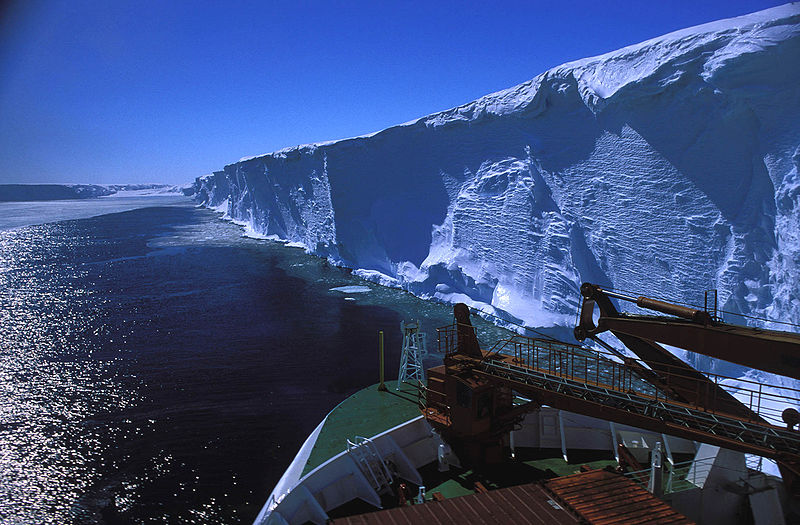
\includegraphics[width=0.7\textwidth]{photos/ice_shelf_edge_hg}

\tiny edge of Ekstr\"om ice shelf, photo Hans Grobe, Polarstern expedition ANT-XX/2
\end{center}
}
\end{frame}


\begin{frame}{SSA stress balance 2}

\begin{columns}
\begin{column}{0.55\textwidth}
SSA also applies reasonably well to ice streams
\begin{itemize}
\item \dots with modest bed topography
\item \dots and weak bed strength
\end{itemize}
\end{column}

\begin{column}{0.45\textwidth}
%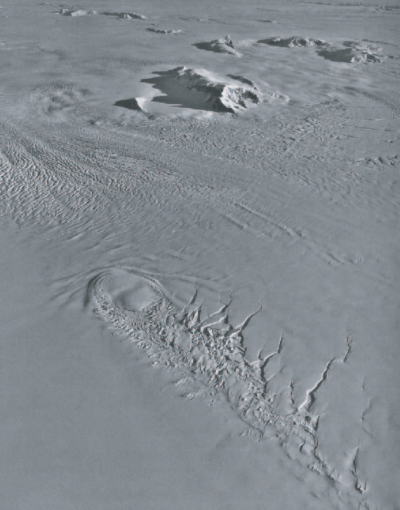
\includegraphics[width=1.0\textwidth]{photos/palmer_land}
%\tiny Palmer Land, Antarctica, photo 131 (Post \& LaChapelle 2000)\cite{PostLaChapelle}
  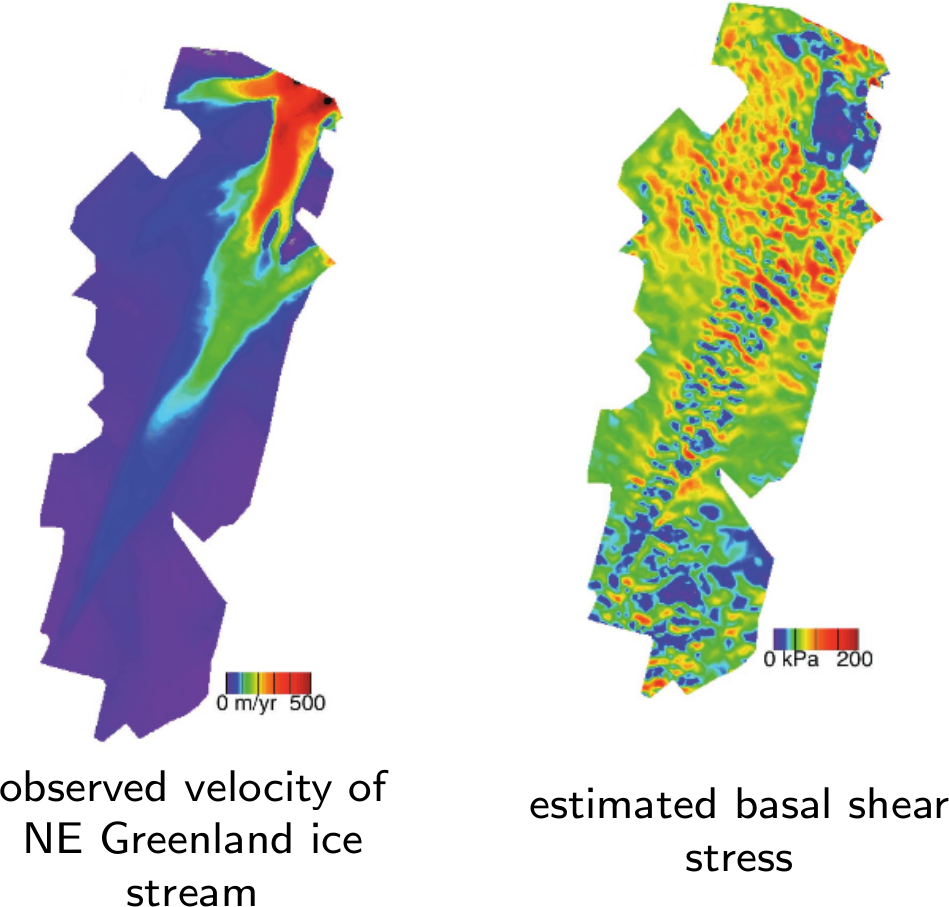
\includegraphics[width=1.0\textwidth]{photos/NEgreenlandJoughin}
\end{column}
\end{columns}

\bigskip\bigskip
\small
\emph{comment}:  energy conservation issues---both ice temperature and basal melt rate---are a major part of ice stream flow modeling [Raymond, 2000]\nocite{Raymondenergy}, \emph{but they are not addressed in these lectures}
\end{frame}


\begin{frame}{what is, \emph{and is not}, an ice stream?}

\begin{columns}
\begin{column}{0.6\textwidth}
\begin{itemize}
\item ice streams have fast flow ($50$ to $>1000 \,\text{m}\,\text{a}^{-1}$) by sliding, with
  \small
  \begin{itemize}
  \item[$\circ$] low bed resistance and
  \item[$\circ$] a critical role of \emph{liquid water} at bed [Clarke, 2005]\nocite{Clarke05}
  \end{itemize}
  \normalsize
\item ``outlet glaciers'' may have the same properties, but they have substantial vertical shear and proportionally less sliding
\item \emph{and} they have lower aspect ratio than ``true'' ice streams
\item \emph{and} some outlet glaciers are really fast, e.g.~Jakobshavn Isbrae
\item thus: \emph{few simplifying assumptions are possible for outlet glaciers}
\item not clear you should use SSA for outlet glaciers
\end{itemize}
\end{column}

\begin{column}{0.4\textwidth}
\mode<presentation>{
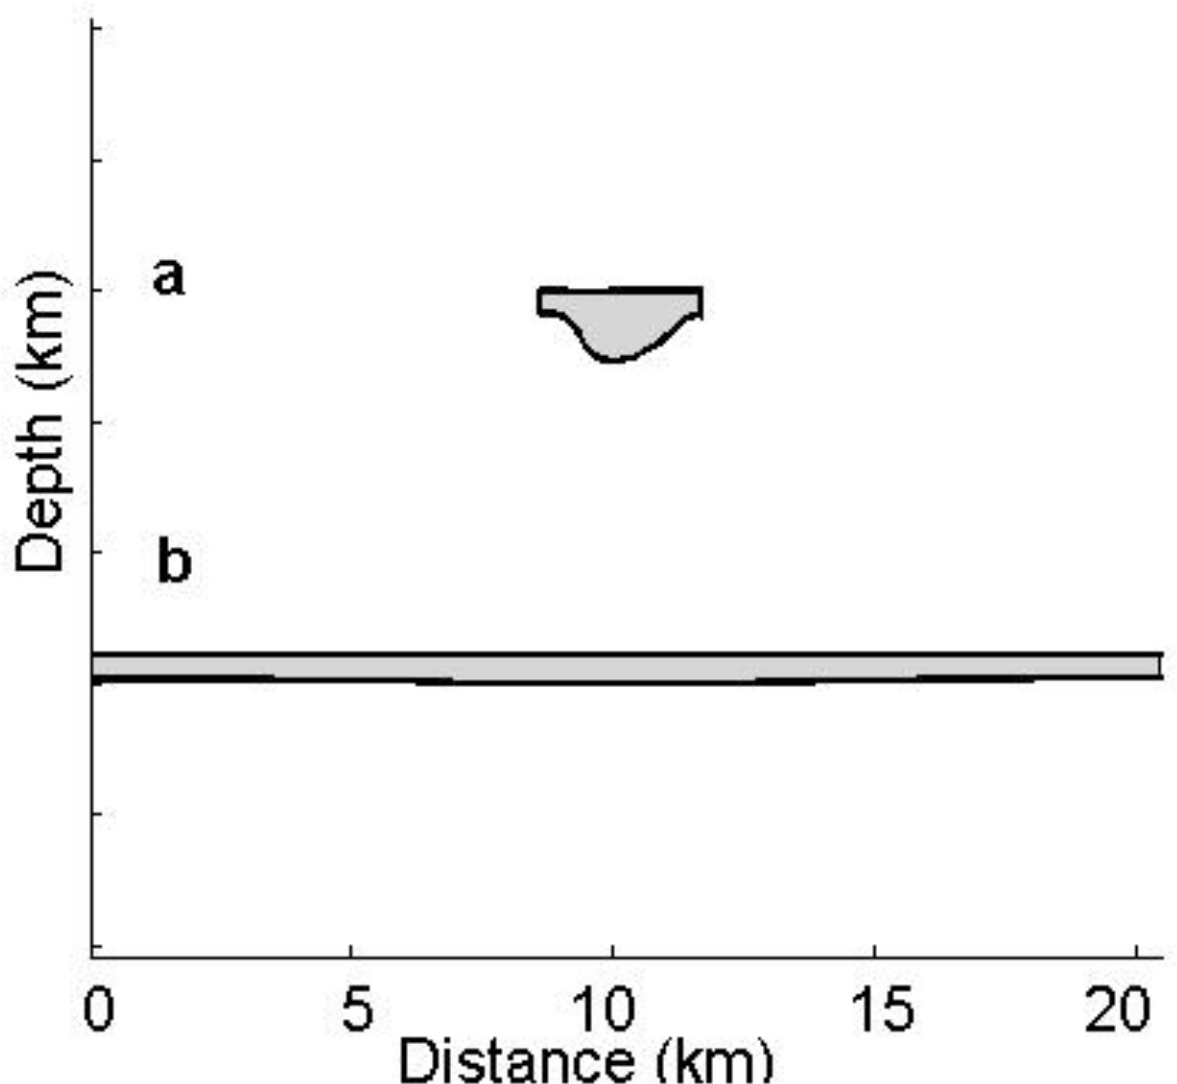
\includegraphics[width=1.0\textwidth]{photos/streamisbrae}

\bigskip
\scriptsize 
Cross sections of Jakobshavns Isbrae (\textbf{a}) and
Whillans Ice Stream (\textbf{b}).  Plotted
without vertical exaggeration in order to better illustrate
the difference between the two types.  (\tiny Figure 1 in [Truffer and Echelmeyer, 2003]\nocite{TrufferEchelmeyer})
}
\end{column}
\end{columns}
\end{frame}


\begin{frame}{stream-to-shelf flow line: notation again}
\begin{center}
  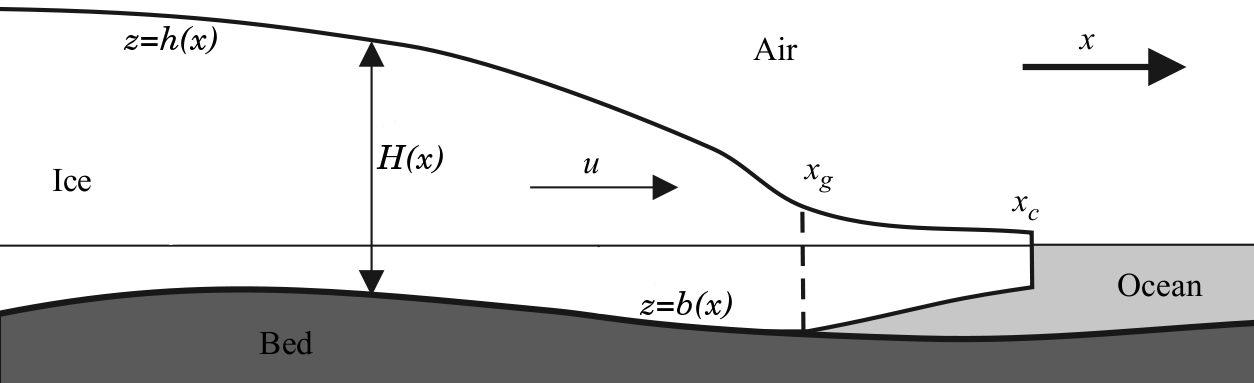
\includegraphics[width=0.96\textwidth]{photos/flowline}

\bigskip
\tiny \emph{figure modified from} [Schoof, 2007]\nocite{SchoofMarine1}
\end{center}
\end{frame}


\begin{frame}{the SSA equation}

\begin{itemize}
\item we will only work in plane flow case
\item we will numerically solve only the stress balance equation which determines the velocity in an ice shelf or ice stream:
\begin{empheq}[box=\fbox]{equation}
  \left({\color{blue}2 A^{-1/n} H |u_x|^{1/n - 1} u_x}\right)_x - C|u|^{m-1}u - \rho g H h_x = 0 \label{ssa}
\end{empheq}
  \begin{itemize}
  \scriptsize
  \item[$\circ$] derived originally by Morland [1987]\nocite{Morland}, MacAyeal [1989]\nocite{MacAyeal}
  \item[$\circ$] references: Weis and others [1999]\nocite{WeisGreveHutter}, Schoof [2006; 2007]\nocite{SchoofStream,SchoofMarine1}
  \normalsize
  \end{itemize}
\item the {\color{blue} blue term} inside parentheses is the vertically-integrated ``longitudinal'' or ``membrane'' stress

%\item two horizontal dimension ($x$ and $y$) version of this equation is significantly harder to solve numerically (Goldberg et al. 2009\cite{Goldbergetal2009})
\item \emph{how to solve this equation numerically}?
\item \emph{how to think about it}?
\end{itemize}
\end{frame}


\begin{frame}{the full monty, with a grounding line}
\label{slide:streamtoshelf}

\small
here is a full flow line context:
\begin{align*}
  u(0) = (\text{given}) \\
  \left.\begin{array}{r}
  \boxed{\left(2 A^{-1/n} H |u_x|^{1/n - 1} u_x\right)_x - C|u|^{m-1}u - \rho g H h_x = 0} \\
  H_t = M - (uH)_x \\
  \rho H \ge \rho_w (-b) \\
  h = H + b
  \end{array}\right\}& \text{ on } 0 < x < x_g \\
  h,u,u_x \text{ continuous at }& x=x_g \\
  \left.\begin{array}{r}
  \boxed{\left(2 A^{-1/n} H |u_x|^{1/n - 1} u_x\right)_x - \rho g (1-\rho/\rho_w) H H_x = 0} \\
  H_t = M - (uH)_x \\
  \rho H < \rho_w (-b)
  \end{array}\right\}& \text{ on } x_g < x < x_c \\
  \left.\begin{array}{r}
  2 A^{-1/n} H |u_x|^{1/n - 1} u_x - \frac{1}{2}\rho (1-\rho/\rho_w) g H^2 = 0 \\
  (\text{a condition describing movement of } x_c)
  \end{array}\right\}& \text{ at } x = x_c
\end{align*}
\small
\begin{itemize}
\item this is the default model in the Marine Ice Sheet Model Intercomparison Project [MISMIP; Schoof and others, 2008]\nocite{MISMIPwebpage}
\item \emph{effectively an open problem}:  what is best numerical treatment of grounding line movement in above model?
\end{itemize}
\end{frame}


\subsection{flow-line ice shelf}

\begin{frame}{exact thickness and velocity for steady ice shelf}


\begin{itemize}
\item we need a more limited goal!
\item \emph{first goal}:  solve the steady state ice shelf in the isothermal, plane flow, and Glen law case
\item for this nice situation, there is a nice result: the thickness and velocity in the ice shelf can be completely determined\footnote{e.g.~[van der Veen, 1985]\nocite{vanderVeen85}} from:
  \begin{enumerate}
  \item ice thickness $H_g$ at the grounding line,
  \item ice velocity $u_g$ at the grounding line,
  \item an integrable (e.g.~constant) surface balance $M(x)$
  \end{enumerate}
\item we do this by-hand on the next slide
\item we will use the by-hand result to:
  \begin{itemize}
  \item[$\circ$] understand the SSA, and
  \item[$\circ$] verify a numerical code
  \end{itemize}
\end{itemize}
\end{frame}


\begin{frame}{exact thickness and velocity for steady ice shelf 2}

\small
  \begin{enumerate}
  \item using flotation criterion $h = (1-\rho/\rho_w) H$, and because of no bed resistance, equation \eqref{ssa} says ``derivative of something $=0$'':
\begin{equation}
  \left(2 A^{-1/n} H |u_x|^{1/n - 1} u_x\right)_x - \left(\frac{1}{2} \rho g (1-\rho/\rho_w) H^2\right)_x = 0  \label{derivequalszero}
\end{equation}
  \item use the calving-front condition to integrate \eqref{derivequalszero}:
\begin{equation}
2 A^{-1/n} H |u_x|^{1/n - 1} u_x - \frac{1}{2} \rho g (1-\rho/\rho_w) H^2 = 0  \label{shelfsteadyu}
\end{equation}
  \item the steady  ($H_t=0$) mass continuity equation can be integrated; here $M=M_0=$constant but some other $M(x)$ are allowed:
\begin{equation}
uH = M_0(x-x_g) + u_g H_g,  \label{shelfsteadyflux}
\end{equation}
  \item multiply \eqref{shelfsteadyu} by $u/H$, replace $uH$ from \eqref{shelfsteadyflux}, assume positive strain rate ($u_x>0$), compute $n$th power
  \item get $u^n u_x = C_s \left(M_0(x-x_g) + u_g H_g\right)^n$, where $C_s$ is known
  \item integrate the last result to find $u(x)$, then return to \eqref{shelfsteadyflux} to find $H(x)$:
\begin{gather*}
u(x)^{n+1} = u_g^{n+1} + \frac{C_s}{M_0} \left[\left(M_0(x-x_g) + u_g H_g\right)^{n+1} - (u_g H_g)^{n+1}\right], \\
H(x) = \frac{M_0(x-x_g) + u_g H_g}{u(x)}
\end{gather*}
  \end{enumerate}
\end{frame}


\begin{frame}{exact thickness and velocity for steady ice shelf 3}

\small
\begin{itemize}
\item Matlab/Octave code \texttt{exactshelf.m} uses shelf length $L=200$ km, and $H_g=500$, $u_g = 50\,\text{m}\,\text{a}^{-1}$
\item computes this shelf geometry and velocity:
  \begin{center}
  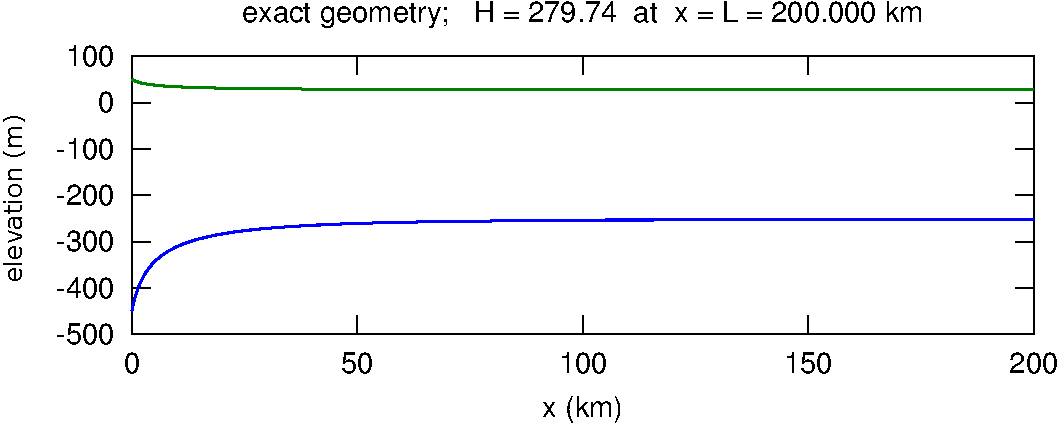
\includegraphics[width=0.7\textwidth]{photos/shelfthk}

  \smallskip
  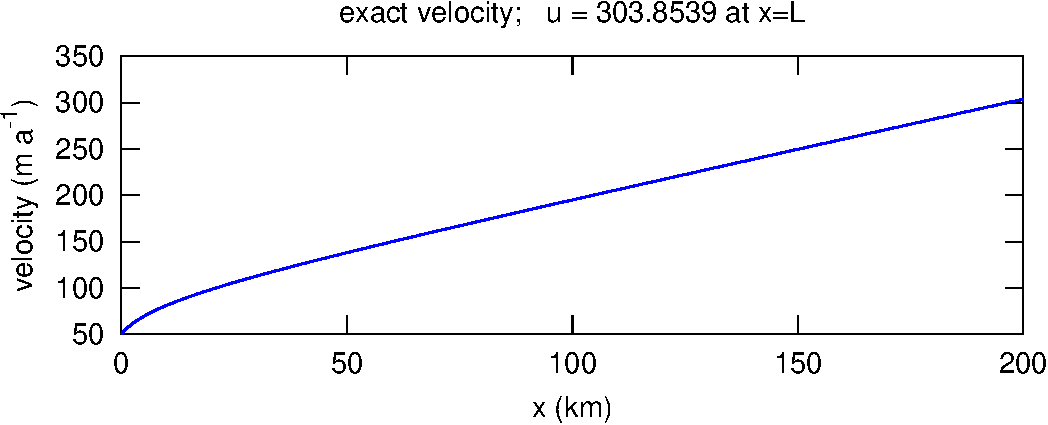
\includegraphics[width=0.7\textwidth]{photos/shelfvel}
  \end{center}
\end{itemize}
\end{frame}


\subsection{numerical solution}


\begin{frame}{numerically solving the SSA}

\begin{itemize}
\item the stress balance is a two-point boundary value problem (BVP) for the velocity $u(x)$:
\small
\begin{gather*}
\left(2 A^{-1/n} H |u_x|^{1/n - 1} u_x\right)_x - C|u|^{m-1}u - \rho g H h_x = 0, \\
\begin{matrix}
\text{\emph{left b.c.}:} & u(x_g) = u_g, \\
\text{\emph{right b.c.}:} & 2 A^{-1/n} H |u_x|^{1/n - 1} u_x - \frac{1}{2}\rho (1-\rho/\rho_w) g H^2 = 0 \text{ at } x = x_c
\end{matrix}
\end{gather*}
\normalsize
\item here we will prescribe the ice geometry, thus both the thickness $H(x)$ and the driving stress $\rho g H h_x$, and we will find the velocity $u(x)$
\item I'll describe the numerical method for a ice shelf \emph{or} ice stream
\item \dots but then I'll give a code \emph{only} for an ice shelf, so $C=0$ and $h=(1-\rho/\rho_w)H$
\end{itemize}
\end{frame}


\begin{frame}{numerically solving the SSA stress balance 2}

\begin{itemize}
\item like most such nonlinear equations, iteration is needed to solve this one
\item red term $\bar \nu = {\color{red} A^{-1/n} |u_x|^{1/n-1}}$ is the ``effective viscosity'':
   $$\left(2 {\color{red} A^{-1/n} |u_x|^{1/n-1}} H u_x\right)_x - C |u|^{m-1} u - \rho g H h_x = 0$$
\item let
   $$W(u_x) = 2 \bar \nu H = 2 A^{-1/n} |u_x|^{1/n-1} H$$
\item \emph{idea}: use old effective viscosity to get new velocity solution, and repeat until the solution is not changing too much and/or the differential equation is nearly-satisfied
\item \emph{idea as algorithm}: from $u^{(k-1)}$, find next values $u^{(k)}$ by solving the \emph{linear} problem
   $$\left(W(u^{(k-1)}_x) u^{(k)}_x\right)_x - C |u^{(k-1)}|^{m-1} u^{(k)} - \rho g H h_x = 0$$
\end{itemize}
\end{frame}


\begin{frame}{numerically solving the SSA stress balance 3}

where do you get an initial guess $u^{(0)}(x)$ for the velocity?
\medskip

\begin{itemize}
\item \emph{for floating ice}, a velocity comes from assuming a uniform strain rate:
   $$u^{(0)} = \gamma (x-x_g) + u_g$$
  \begin{itemize}
  \item[$\circ$]  for example: $\gamma$ is the value of $u_x$ found from the calving front stress imbalance and $u_g$ is the known velocity at the grounding line
  \end{itemize}
\item \emph{for grounded ice}, a velocity comes from assuming the ice is held by basal resistance only:
   $$u^{(0)} = \left(-C^{-1} \rho g H h_x\right)^{1/m}$$
\end{itemize}
\end{frame}


\begin{frame}{solving the ``inner'' linear problem}
\begin{itemize}
\item reset $x$ interval to be $0 < x < L$, instead of $x_g < x < x_c$
\item abstract the problem to a linear BVP:
   $$\left(W(x)\, u_x\right)_x - \alpha(x)\, u = \beta(x)$$
with boundary conditions
   $$u(0) = V, \qquad  u_x(L) = \gamma$$
\item $W(x)$, $\alpha(x)$, $\beta(x)$ are all known functions in this abstract problem
\item for the nonlinear SSA equation, both $W(x)$ and $\alpha(x)$ will come from the previous iteration
\item $W(x)$ is needed on the staggered grid, for $O(\Delta x^2)$ accuracy, as with time-dependent diffusion problem earlier
\item $\alpha(x),\beta(x)$ are needed on regular grid
\end{itemize}
\end{frame}


\begin{frame}{solving the ``inner'' linear problem 2}

\begin{itemize}
\item indices $j=1,2,\dots,J+1$
\item equal-spaced grid $x_1,x_2,\dots,x_{J+1}$, where $x_1 = 0$ and $x_{J+1} = L$
\item an approximation of the abstracted problem is:
$$\frac{W_{j+1/2} (u_{j+1} - u_j) - W_{j-1/2} (u_{j} - u_{j-1})}{\Delta x^2} - \alpha_j u_j \stackrel{\ast}{=} \beta_j$$
\item $u_1 = V$ given
\item for right-hand boundary condition ``$u_x(L)=\gamma$'':
  \begin{itemize}
  \item[$\circ$] introduce notional point $x_{J+2}$
  \item[$\circ$]
    $$\frac{u_{J+2} - u_J}{2 \Delta x} = \gamma$$
  \item[$\circ$] using equation $\ast$ in $j=J+1$ case, eliminate $u_{J+2}$ variable ``by-hand'' [Morton and Mayers, 2005]\nocite{MortonMayers}
  \end{itemize}
\end{itemize}
\end{frame}


\begin{frame}{solving the ``inner'' linear problem 3}

\scriptsize
\begin{itemize}
\item so abstract linear system has matrix-vector form `` $A \mathbf{x} = \mathbf{b}$ '':
$$
\begin{bmatrix}
1 &  &  &  &  \\
W_{3/2} & A_{22} & W_{5/2} &  &  \\
 & W_{5/2} & A_{33} &  &  \\
 &  & \ddots & \ddots &  \\
 &  & W_{J-1/2} & A_{JJ} & W_{J+1/2} \\
 &  &  & A_{J+1,J} & A_{J+1,J+1} \\
\end{bmatrix}\,
\begin{bmatrix}
u_1 \\ u_2 \\ u_3 \\ \vdots \\ u_J \\ u_{J+1}
\end{bmatrix}
=
\begin{bmatrix}
V \\ \beta_2 \Delta x^2 \\ \beta_3 \Delta x^2 \\ \vdots \\ \beta_J \Delta x^2 \\ b_{J+1}
\end{bmatrix}
$$
\item with diagonal entries  ($j=2,3,\dots,J$)
$$A_{jj} = -(W_{j-1/2}+W_{j+1/2}+\alpha_j \Delta x^2)$$
\item with special cases in last equation:
$$A_{J+1,J} = W_{J+1/2}+W_{J+3/2}$$
$$A_{J+1,J+1} = -(W_{J+1/2}+W_{J+3/2}+\alpha_{J+1}\Delta x^2)$$
$$b_{J+1} = -2 \gamma \Delta x W_{J+3/2} + \beta_{J+1} \Delta x^2$$
\item this is a \emph{tridiagonal} system
\end{itemize}
\end{frame}


\begin{frame}{solving the ``inner'' linear problem 4}
\label{slide:flowlinecode}

\minput{flowline}
\end{frame}


\begin{frame}{solving the ``inner'' linear problem 5}

\begin{itemize}
\item before proceeding to solve nonlinear SSA problem, we can test the ``abstracted'' code \texttt{flowline.m}
\item \dots by ``manufacturing'' solutions as in code \texttt{testflowline.m} \quad \scriptsize (not shown) \normalsize
\item \emph{results}: \quad works pretty well! converges at optimal rate $O(\Delta x^2)$
\end{itemize}

\begin{center}
  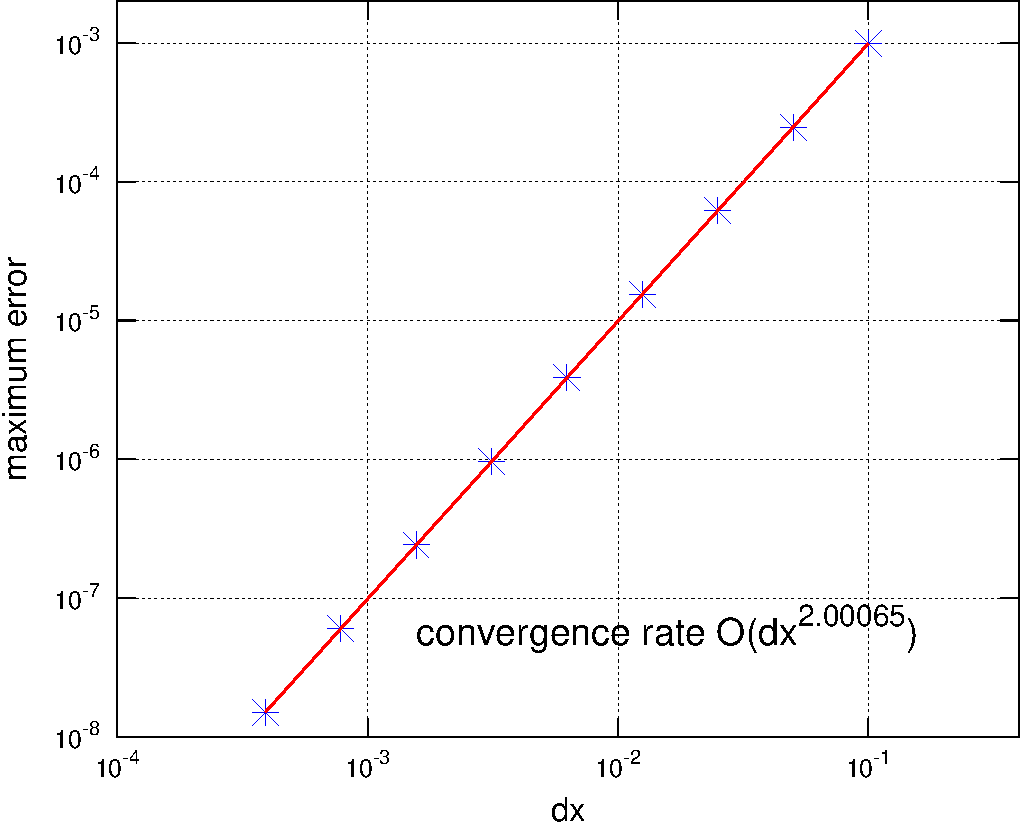
\includegraphics[width=0.65\textwidth]{photos/convanalysis}
\end{center}
\end{frame}


\begin{frame}{numerical solution to SSA}

\minputtiny{ssaflowline}
\end{frame}


\begin{frame}{\emph{numerical} thickness and velocity for steady ice shelf}

\begin{itemize}
\item first: let's numerically solve the problem for which we know exact answer
\item here use very coarse 10 km grid
\end{itemize}

\begin{center}
  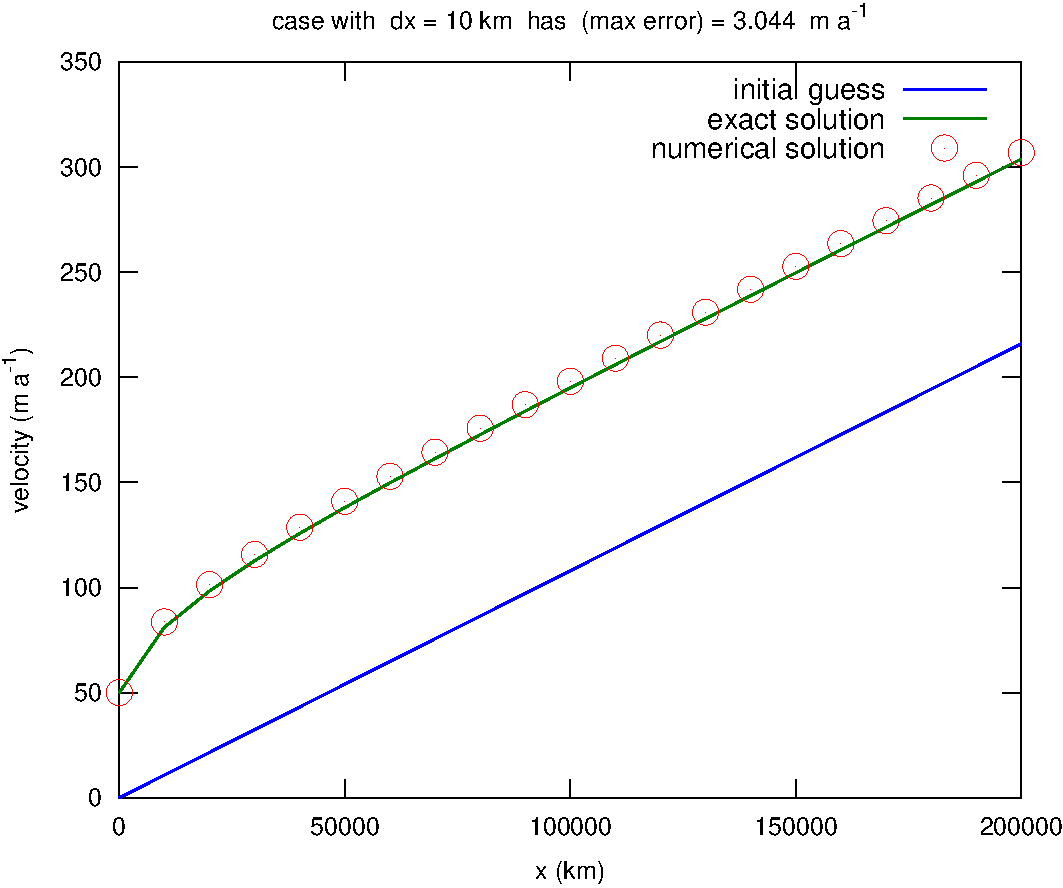
\includegraphics[width=0.7\textwidth]{photos/shelfnumsoln}
\end{center}
\end{frame}


\begin{frame}[fragile]
  \frametitle{did we make any mistakes?}

\begin{itemize}
\item this does convergence analysis of \mname{ssaflowline.m}:

\scriptsize
\begin{verbatim}
J = [50 100 200 400 800 1600 3200];   dxkm = 200.0 ./ J;              
for j=1:length(J)
  [av,maxerr(j)] = testshelf(J(j));   % calls ssaflowline.m
end
loglog(dxkm,maxerr,'0-','markersize',16)
\end{verbatim}
\normalsize
\item goal is to see velocity error shrink by rate built-into our finite differences, namely at nearly the optimal rate $O(\Delta x^2)$
\item by this standard, we likely made no mistakes!
\end{itemize}

\begin{center}
  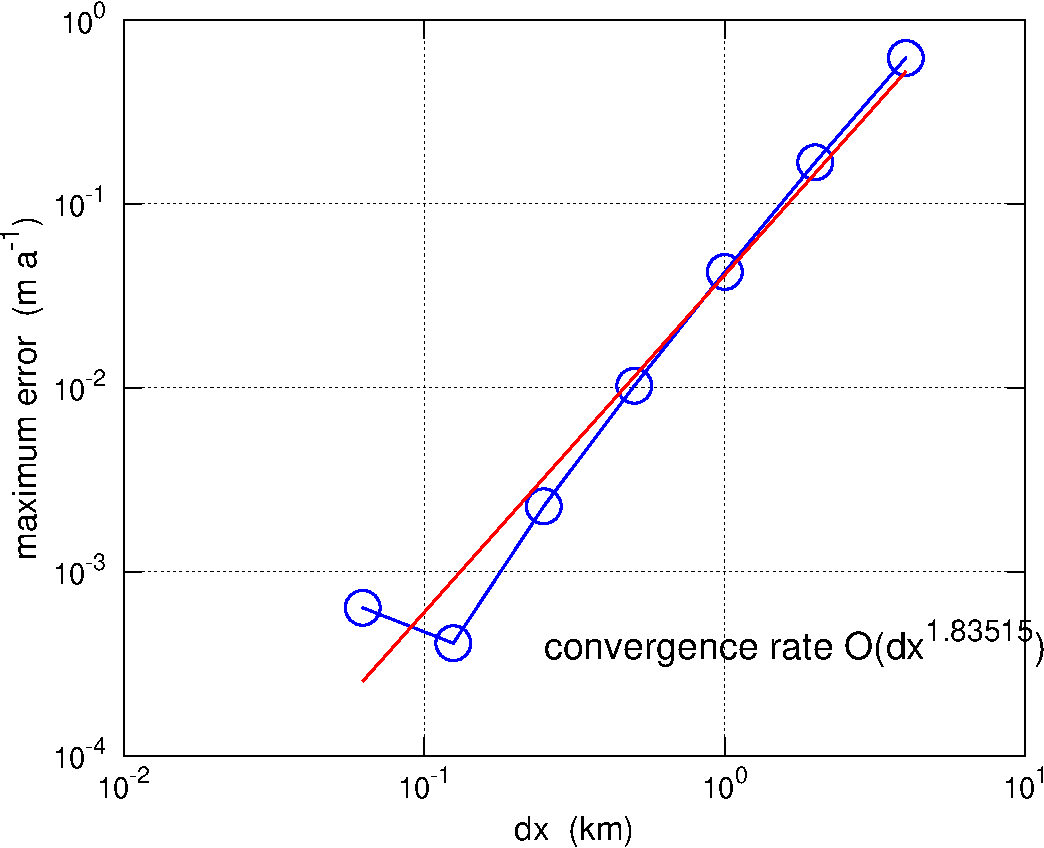
\includegraphics[width=0.55\textwidth]{photos/shelfconv}
\end{center}
\end{frame}


\begin{frame}{realistic ice shelf modeling}

\small
\begin{itemize}
\item flow lines (1D) are never very realistic \dots
\item ``diagnostic'' (= fixed geometry) ice shelf modeling in two horizontal variables (2D) has been quite successful
\item solve an \emph{elliptic} PDE boundary value problem
\item velocity measurements are available for validation
  \begin{itemize}
  \scriptsize
  \item[$\circ$] Ross ice shelf example based on [RIGGS; Bentley, 1974]\nocite{RIGGS1} data below: model (\alert{red} arrows) vs observations (\textbf{black} arrows)
  \item[$\circ$] this is PISM but many models can do it [MacAyeal and others, 1996]\nocite{MacAyealetal}
  \item[$\circ$] something of a mystery why regular grid methods do well!
  \small
  \end{itemize}
\end{itemize}

\begin{center}
  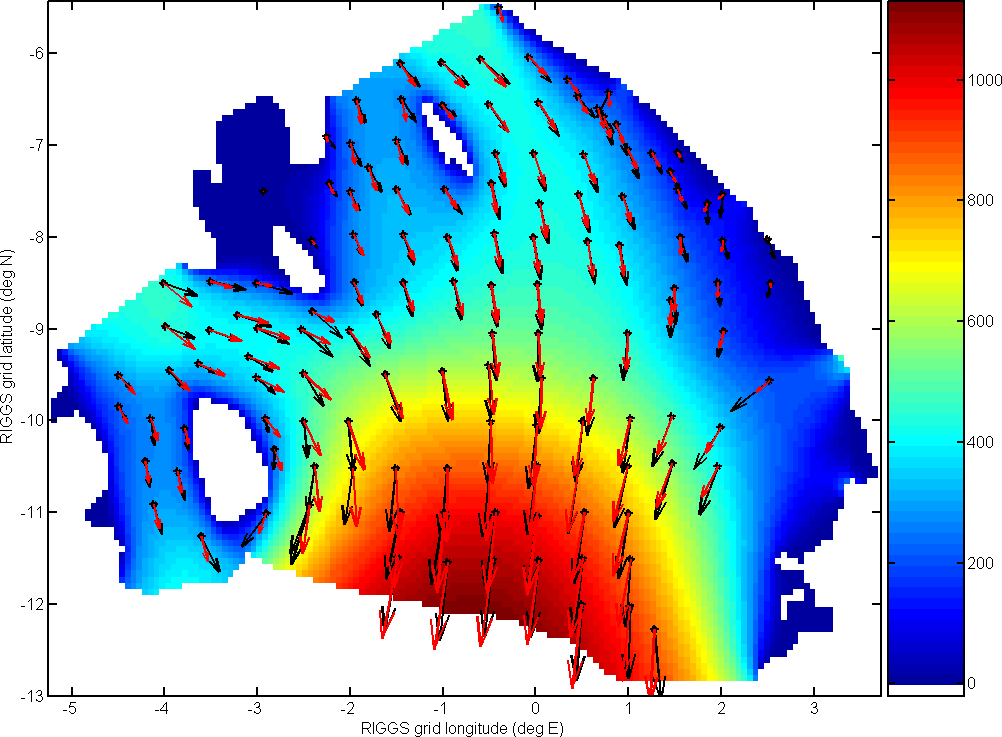
\includegraphics[width=0.6\textwidth]{photos/PISM_ross_speeds}
\end{center}
\end{frame}


\subsection{scaling up}

\begin{frame}{numerical solution of SSA: a summary}

\begin{itemize}
\item SSA and Blatter [1995]\nocite{Blatter} stress balance equations each
   \begin{itemize}
   \item[$\circ$]  determine horizontal velocity from geometry and b.c.s
   \item[$\circ$]  are nonlinear problems: require iterative linearization
   \item[$\circ$]  each ``inner'' linear problem has a sparse pattern
      \begin{itemize}
      \item[$\ast$] tridiagonal in SSA flow-line (1D) case here
      \item[$\ast$] much less structured in SSA 2D, Blatter 2D, and Blatter 3D cases
      \end{itemize}
   \end{itemize}
\item the Stokes stress balance is much harder because incompressibility must be handled explicitly
\item a wise numerical modeler would give the sparse linear problem to a numerical linear algebra software package:
  \begin{itemize}
  \item[$\circ$]  \Matlab/\Octave, \emph{LAPACK}, \emph{PETSc}, \emph{Trilinos}, \dots
  \item[$\circ$]  generally: modularize your code and \emph{test the parts separately}!
  \end{itemize}
\item \emph{comment} on mass continuity:  
  \begin{itemize}
  \item[$\circ$]  the mass continuity PDE ``$H_t = M - \Div\left(\bar \bu H\right)$'' is \emph{not} very diffusive if the source of $\bar \bu$ is SSA or Blatter,
  \item[$\circ$]  and there is \emph{not much theory} to guide how to solve such a generic transport problem
  \end{itemize}
\end{itemize}
\end{frame}


\begin{frame}{scaling-up the numerical solution of stress balances}

\begin{itemize}
\item all stress balance equations used for ice flow modeling are nonlinear equations for velocity $\bu$ in the form
	$$\bbF(\bu) = 0$$
\vspace{-0.1in}
\item the ``residual'' $\bbF$ involves various partial derivatives, nonlinear operations, and additional fields (e.g.~thickness)
\item SSA and Blatter stress balance equations can be written in form
	 $$\bA(\bu)\,\bu = \bg$$
\vspace{-0.15in}
  \begin{itemize}
  \item[$\circ$]  where $\bA$ is a nonlinear function of $\bu$,
  \item[$\circ$]  and $\bA(\bu)$ acts linearly on $\bu$
  \end{itemize}
\item we have already treated the SSA in the second way
\item both forms are nonlinear, elliptic PDEs
\item Newton [1669] knew a way of solving nonlinear equations!
\end{itemize}
\end{frame}


\begin{frame}{scaling-up the numerical solution of stress balances 2}

\begin{itemize}
\item the iteration scheme we have used for SSA is ``Picard'':
	$$\bA(\bu^{(k-1)})\,\bu^{(k)} = \bg$$
\vspace{-0.2in}
  \begin{itemize}
  \item[$\circ$] this iteration converges linearly, if it converges:  $\|\bu^{(k+1)} - \bu^{(k)}\| \le \gamma \|\bu^{(k)} - \bu^{(k-1)}\|$, where $0<\gamma<1$
  \item[$\circ$] it can be robust, but it is not fast
  \end{itemize}	
\item Newton's method (e.g.~[Press and others, 1992])\nocite{Pressetal} also solves $\bbF(\bu) = 0$ iteratively, but by linearization:
\begin{gather*}
J(\bu^{(k-1)})\,\bw = - \bbF(\bu^{(k-1)}), \\
\bu^{(k)} = \bu^{(k-1)} + \bw
\end{gather*}
\vspace{-0.1in}
where
   $$J(\bu)_{ij} = \frac{\partial \bbF(\bu)_i}{\partial \bu_j} \qquad \text{is the \emph{Jacobian} of } \bbF$$
\vspace{-0.1in}
  \begin{itemize}
  \item[$\circ$] this iteration converges quadratically, if it converges:  $\|\bu^{(k+1)} - \bu^{(k)}\| \le C \|\bu^{(k)} - \bu^{(k-1)}\|^2$
  \item[$\circ$] much faster!
  \end{itemize}	
\end{itemize}
\end{frame}


\begin{frame}{scaling-up the numerical solution of stress balances 3}

\begin{itemize}
\item big computers still take a long time to solve SSA equations when grids are $\sim 2$ km for Greenland
  \begin{itemize}
  \item[$\circ$] Antarctica is $10\times$ the area, and that much worse!
  \end{itemize}
\item there are various numerical paradigms for discretizing (finite difference, finite element, spectral, \dots), but choosing among these is \emph{not} the major scalability issue
\item effective scalability of 3D stress balances (e.g.~Blatter \& Stokes) at high spatial resolution, on large parallel machines \textbf{requires}:
  \begin{itemize}
  \item[$\circ$] the ``inner'' linear solve must be iterative--not by Gaussian elimination---and must be preconditioned
  \item[$\circ$] the ``outer'' nonlinear iteration must offer faster-than-linear convergence
  \item[$\circ$] because the exact Jacobian is too hard to evaluate---certainly so with coupling to other physics (e.g.~thermo-)---the method must allow approximated Jacobians
  \end{itemize}
\item this is the promise of ``preconditioned matrix-free Newton-Krylov'' (e.g.~[Knoll and Keyes, 2004]\nocite{KnollKeyes2004}) as a paradigm for big, nasty nonlinear problems
\end{itemize}
\end{frame}


\begin{frame}{scaling-up the numerical solution of stress balances 4}

\begin{columns}
\begin{column}{0.5\textwidth}
\begin{itemize}
\small
\item the PETSc [Balay and others, 2010]\nocite{petsc-user-ref} library has evolved into a Newton-Krylov toolkit \quad $\to$
\item my online materials turn \texttt{ssaflowline.m} into a C PETSc example \texttt{ssaflowline.c}:
  \begin{itemize}
  \small
  \item[$\circ$] parallel over an arbitrary number of processors
  \item[$\circ$] uses Newton method (or Picard)
  \item[$\circ$] try matrix-free, different preconditioners, \dots
  \item[$\circ$] result from \texttt{ssaflowline.c} is at lower-right:
     \begin{itemize}
     \scriptsize
     \item[$\ast$] evidence of super-linear convergence from Newton method
     \item[$\ast$] on coarsest grids, $10$ or $100$ points, get rapid convergence to $10^{-13}$ of the initial residual norm
     \end{itemize}
  \end{itemize}
\end{itemize}
\end{column}
\begin{column}{0.6\textwidth}
\begin{center}
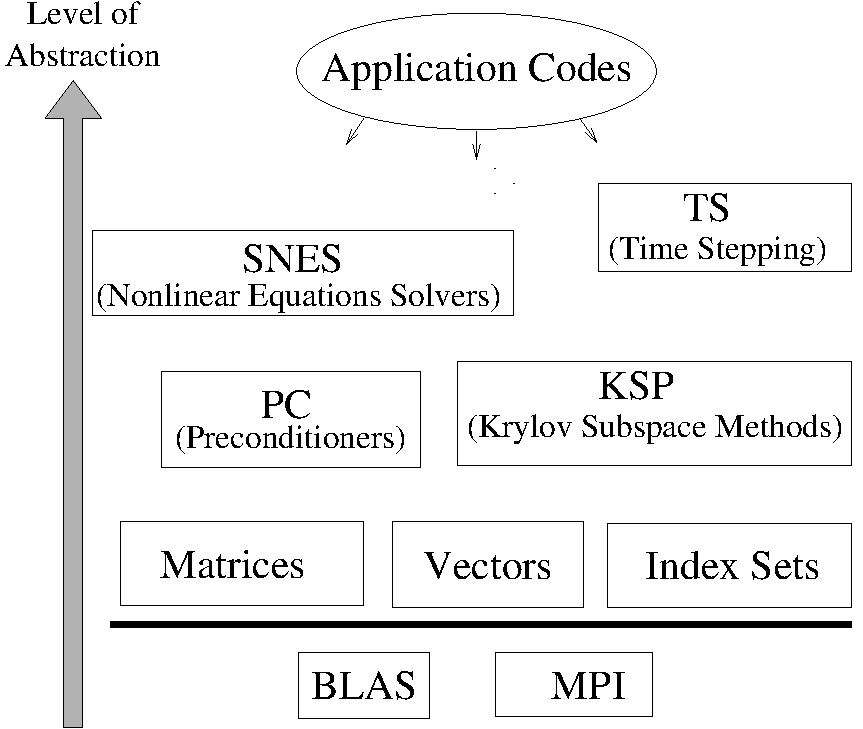
\includegraphics[width=0.65\textwidth]{photos/petscwww}
\end{center}

\begin{center}
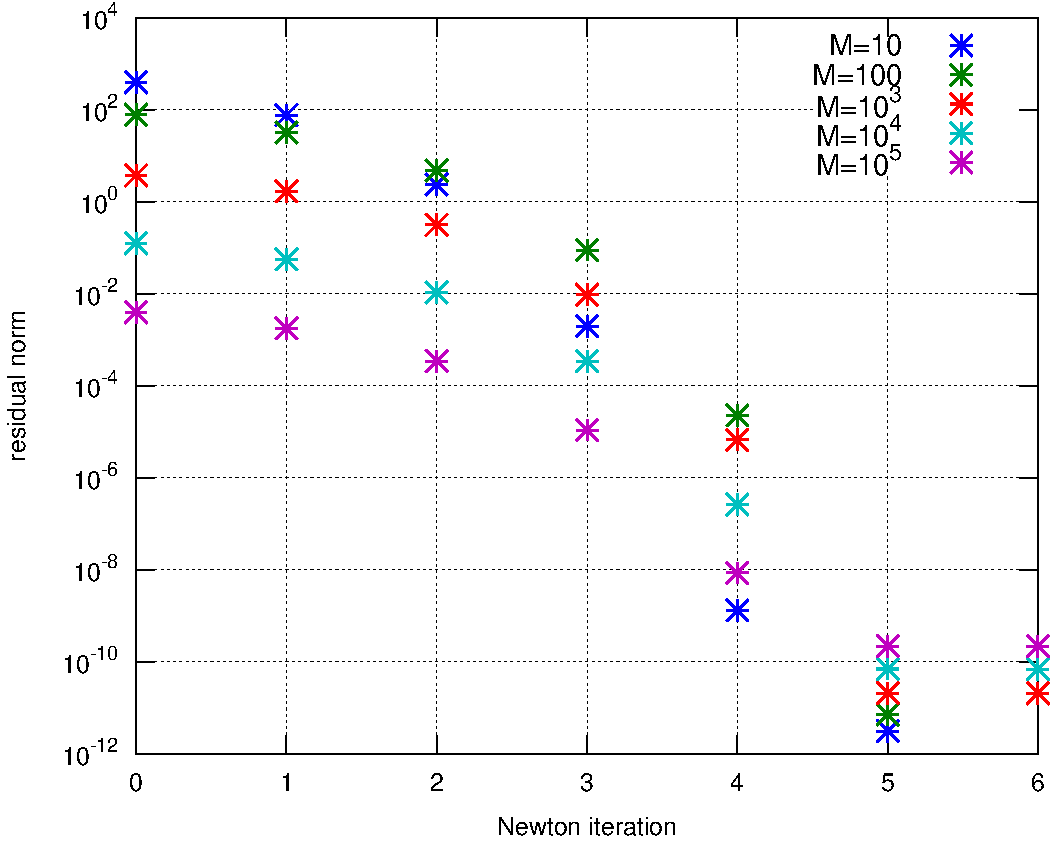
\includegraphics[width=0.85\textwidth]{petsc/notes/quadconv}
\end{center}

\scriptsize

\end{column}
\end{columns}

\end{frame}
